\documentclass[Royal,times,sageh]{sagej}

\usepackage{moreverb,url,natbib, multirow, tabularx}
\usepackage[colorlinks,bookmarksopen,bookmarksnumbered,citecolor=red,urlcolor=red]{hyperref}



% tightlist command for lists without linebreak
\providecommand{\tightlist}{%
  \setlength{\itemsep}{0pt}\setlength{\parskip}{0pt}}



\usepackage[linesnumbered,lined,boxed,commentsnumbered]{algorithm2e}
\usepackage{booktabs}
\usepackage{longtable}
\usepackage{array}
\usepackage{multirow}
\usepackage{wrapfig}
\usepackage{float}
\usepackage{colortbl}
\usepackage{pdflscape}
\usepackage{tabu}
\usepackage{threeparttable}
\usepackage{threeparttablex}
\usepackage[normalem]{ulem}
\usepackage{makecell}
\usepackage{xcolor}


\begin{document}


\setcitestyle{aysep={,}}

\title{A geo-referenced micro-data set of real estate listings for the
three largest Spanish cities}

\runninghead{Rey-Blanco \emph{et al}.}

\author{D. Rey-Blanco\affilnum{1}, P. González-Arbues\affilnum{1}, F.
López\affilnum{2}, A. Páez*\affilnum{4}}

\affiliation{\affilnum{1}{Idealista, Plaza de las Cortes 5, 28014
Madrid, Spain}\\\affilnum{2}{Facultad de CC de la Empresa, C/ Real, 3.
30201 Cartagena, Murcia, Spain}\\\affilnum{3}{School of Earth,
Environment and Society, McMaster University, 1280 Main St W, Hamilton,
Ontario L8S 4K1 Canada}}

\corrauth{Antonio Páez, School of Earth, Environment and Society,
McMaster University, 1280 Main St W, Hamilton, Ontario L8S 4K1 Canada.}

\email{\href{mailto:paezha@mcmaster.ca}{\nolinkurl{paezha@mcmaster.ca}}}

\begin{abstract}
This data article shares an open data product with big geo-referenced
micro-data sets of 2018 real estate listings in Spain. These data were
originally published on idealista.com real estate website. The
observations are obtained for the three largest Spanish cities: Madrid
(n = 94,815 observations), Barcelona (n = 61,486 observations) and
Valencia (n = 33,622 observations). The data sets include the
coordinates of properties (latitude and longitude), asking prices of
each listed dwelling, and several variables of indoor characteristics.
The listings were enriched with official information from the Spanish
cadastre (e.g.~built quality materials grade) plus other relevant
geographical features such as distance to urban points of interest.
Along with real estate listings, the data product also includes
neighborhood boundaries for each city. The data product is offered in
the form of a fully documented R package. This open data product is
available for scientific and educational purposes, in particular for
geo-spatial studies.
\end{abstract}

\keywords{Housing market; idealista.com; geo-referenced data; point
level data; open data; hedonic price analysis; Spain}

\maketitle

\hypertarget{introduction}{%
\section{Introduction}\label{introduction}}

The interest about the determinants of housing market and housing prices
has been a growing research area in the last decades, with a vast
literature both theoretical as well as empirical. Include the spatial
component to analyze the real state market, and in general the
incorporate geographic variables, has been significant improvements in
the understanding of this market. But to really understand the
determinants of housing market it is essential to have information/data
at level-point. Therefore, it is increasingly common that the spatial
analysis to be development in urban environment with geo-referenced
micro-data sets \citep[e.g.][]{lopez2015, crespo2013local}. But on the
other hand, the availability of this type of open data at point level is
limited and not to much data set contain latitude/longitude coordinates
of each dwelling. In some cases the researchers it has had to resort to
web scraping processes in order to obtain large volumes of information
that allow get robust analysis
\citep{gupta2022take, arbia2020spatial, Li2019, lopez2015}. These web
scraping processes can include a lot of missing data, download errors,
duplicate records, etc. Furthermore, in general the authors of this
researches do not share the data sets.

In the same vein, in the last years there are a growing interest in open
data in geography and data science
\citep{arribasl2021editorial, arribas2021} and in general by the
reproducible or replicable research \citep{paez2021open}. But to make
open science is necessary have free software and open data. While great
efforts have been made to make free software available to researchers
(e.g.~R or Python), not much data is out in the open. In the particular
case of the real estate market, to our knowledge, no to much open
micro-data set of housing markets are available.

To overcome these limitations, this paper present a sort description of
the an open micro-data set of a geo-referenced dwelling listings. The
data has been provided by Idealista
company\footnote{Idealista is the major real estate listing website in Spain, and present in other southern european countries as Italy and Portugal}
and contain information of 189,923 dwelling localized in the three major
Spanish cities. To the date, this data product is the bigger open
geo-referenced data set of housing market in Spain. Moreover, note that
the data set is supply directly by Idealista and therefore is clean and
free of download errors. The listings has been enriched with official
information from the Spanish cadastre plus other relevant geographical
features such as distance to urban points of interest. The data set is
distributed in the form of an \texttt{R} package, named
\textbf{idealista18} that can be accessed at Github
repository\footnote{The direct URL to the Github repository is https://github.com/paezha/idealista18}.

\hypertarget{data-description}{%
\section{Data description}\label{data-description}}

The open data set `idealista18' is R package composed of nine objects,
three objects for each of the three main Spanish cities: Barcelona,
Madrid and Valencia. For each city, dwelling listings, neighborhood
polygons and a set of points of interest (POI) has been included in the
R package. The next subsections describe each object. A full description
of the data is available in the helps of the package.

\hypertarget{dwelling-listings}{%
\subsection{Dwelling listings}\label{dwelling-listings}}

The dwelling listing of each city, include a set of characteristics of
each dwelling that was published on idealista real state website
(\url{https://www.idealista.com/}) and are included in `idealista18'
package as an sf object \citep{Pebesma}. The data set corresponding to
each city is named with the name of the city followed by '\_Sale'
(e.g.~Madrid\_Sale) and include a total of 42 variables. Each sf objects
contains the complete set of listings, corresponding to the four
quarters of year 2018. The record counts for each city in 2018 are:
94,815 listings for Madrid, 61,486 for Barcelona and 33,622 for
Valencia. Table \ref{tab:number-ads} show the number of dwelling listing
ads included in the data set for city and quarter. Note that is possible
that the same dwelling can be found in more than one period when a
property listed for sale in one quarter was sold in a subsequent
quarter. The variable ASSETID, included in the sf objects is the unique
identifier of the dwelling.

\begin{table}[ht]
\centering
\begin{tabular}{>{\raggedright\arraybackslash}p{4em}>{\raggedleft\arraybackslash}p{3em}cccc}
  \hline
City & First & Second  & Thirdr & Fourth & Total ads \\ 
  \hline
Barcelona & 17826 & 7951 & 12375 & 23334 & 61486 \\ 
  Madrid & 21920 & 12652 & 15973 & 44270 & 94815 \\ 
  Valencia & 9305 & 4655 & 5644 & 14018 & 33622 \\ 
   \hline
\end{tabular}
\caption{Number of dwelling  listing ads for each city and quarter. \label{tab:number-ads}} 
\end{table}

Each record of the dwelling listing contains a set of indoor
characteristics supplied by advertiser in the Idealista web (e.g.~price,
surface, rooms, basic features, etc) including the exact localization of
the dwelling (see Section \protect\hyperlink{anonymizing}{Anonymizing
the data set}). Table \ref{tab:variables} list some of the main indoor
variables included in the dwelling listing with a short description and
the mean value of each variable. This dwelling listing was enriched with
a number of additional attributes from the Spanish cadastre
\citep{Catastro}. Cadastral information is described in Table
\ref{tab:variables}, including the the prefix CAD in the variable name.
Cadastral features assignment is done by assigning the features of the
nearest parcel to the coordinates. The year of construction of dwelling
(CONSTRUCTIONYEAR) supply by the advertiser was revised given that the
year of construction are entered by users in the web site and therefore
subject to errors and incomplete data (a 40\% missing rate). To solve
this issue we include an alternative variable (CADCONSTRUCTIONYEAR)
assign cadastral construction year from the nearest cadastral parcel
whenever value has an outstanding value (date is after publication date
or year of construction is before 1500) or when the value supply by the
advertiser was missing. Additionally, the distance of each dwelling to
three urban points of interest was included in the dwelling listing:
distance to city center, distance to the closed metro station and
distance to the main street (Diagonal street for Barcelona, Castellana
street for Madrid and Blasco Ibañez street for Valencia). The last rows
of Table \ref{tab:variables} show the mean values of this variables.

\begin{table}[ht]
\centering
\fontsize{8}{10}\selectfont
\begin{tabular}{>{\raggedright\arraybackslash}p{13em}>{\raggedright\arraybackslash}p{14em}ccc}
  \hline
Variable & Sort Description & Barcelona & Madrid & Valencia \\ 
  \hline
PRICE & Asking price & 395770.58 & 396110.11 & 199678.31 \\ 
  UNITPRICE & Asking price per m\verb|^|2 (euros) & 4044.86 & 3661.05 & 1714.54 \\ 
  CONSTRUCTEDAREA & Surface (m\verb|^|2) & 95.46 & 101.40 & 108.95 \\ 
  ROOMNUMBER & Number of bedrooms & 2.86 & 2.58 & 3.07 \\ 
  BATHNUMBER & Number of bathrooms & 1.52 & 1.59 & 1.59 \\ 
  CONSTRUCTIONYEAR & Construction year (advertiser) & 1952.58 & 1964.69 & 1969.43 \\ 
  CADCONSTRUCTIONYEAR & Construction year (cadastre) & 1952.19 & 1965.70 & 1970.55 \\ 
  CADMAXBUILDINGFLOOR & Max build floor & 6.85 & 6.38 & 7.04 \\ 
  CADDWELLINGCOUNT & Dwelling count in the building & 28.56 & 39.19 & 36.83 \\ 
  CADASTRALQUALITYID & Cadastral quality. 0 Best-10 Worst & 4.31 & 4.85 & 5.34 \\ 
  DISTANCE\_TO\_CITY\_CENTER & Distance to city center & 2.80 & 4.49 & 2.09 \\ 
  DISTANCE\_TO\_METRO & Distance to subway station & 0.27 & 0.48 & 0.64 \\ 
  DISTANCE\_TO\_(MAINSTREET) & Distance to main street & 1.77 & 2.68 & 2.07 \\ 
   \hline
\end{tabular}
\caption{List, sort description and mean of the main quantitative variables included in the dwelling listing for the three Spanish cities. See the help facility in the \textbf{idealista18} R package for details and formal definitions. Some variables has been excluded of this table for save space, check the full list in  \textbf{idealista18} R package. \label{tab:variables}} 
\end{table}

In addition to the variables listed in Table \ref{tab:variables} the sf
object include a set of dummy variables with information abour basic
characteristics of the dwelling. Table \ref{tab:Dummy-variables} show
the more relevant variables included in the sf object.

\begin{table}[ht]
\centering
\fontsize{8}{10}\selectfont
\begin{tabular}{>{\raggedright\arraybackslash}p{12em}>{\raggedright\arraybackslash}p{14em}ccc}
  \hline
Variable & Sort Description & Barcelona & Madrid & Valencia \\ 
  \hline
HASTERRACE & =1 if has terrace & 0.33 & 0.36 & 0.25 \\ 
  HASLIFT & =1 if has lift & 0.74 & 0.70 & 0.79 \\ 
  HASAIRCONDITIONING & =1 if has air conditioning & 0.47 & 0.45 & 0.47 \\ 
  HASPARKINGSPACE & =1 if has parking & 0.08 & 0.23 & 0.17 \\ 
  HASNORTHORIENTATION & =1 if has north orientation & 0.13 & 0.11 & 0.13 \\ 
  HASSOUTHORIENTATION & =1 if has south orientation & 0.31 & 0.24 & 0.19 \\ 
  HASEASTORIENTATION & =1 if has east orientation & 0.24 & 0.20 & 0.25 \\ 
  HASWESTORIENTATION & =1 if has west orientation & 0.16 & 0.15 & 0.15 \\ 
  HASBOXROOM & =1 if has boxroom & 0.12 & 0.26 & 0.13 \\ 
  HASWARDROBE & =1 if has wardrobe & 0.30 & 0.57 & 0.53 \\ 
  HASSWIMMINGPOOL & =1 if has swinningpool & 0.03 & 0.15 & 0.07 \\ 
  HASDOORMAN & =1 if has doorman & 0.08 & 0.25 & 0.05 \\ 
  HASGARDEN & =1 if has garden & 0.04 & 0.18 & 0.06 \\ 
  ISDUPLEX & =1 if is duplex & 0.03 & 0.03 & 0.02 \\ 
  ISSTUDIO & =1 if is studio & 0.02 & 0.03 & 0.01 \\ 
  ISINTOPFLOOR & =1 is in the top floor & 0.02 & 0.02 & 0.01 \\ 
  BUILTTYPEID\_1 & =1 if is new contruction & 0.01 & 0.03 & 0.03 \\ 
  BUILTTYPEID\_2 & =1 is second hand to be restored & 0.17 & 0.19 & 0.13 \\ 
  BUILTTYPEID\_3 & =1 is second hand good conditions & 0.82 & 0.78 & 0.83 \\ 
   \hline
\end{tabular}
\caption{List of dummy variables, sort description and ratio of dwelling with the specific characteristic. See the help facility in the \textbf{idealista18} R package for details and formal definitions. Some dummy variables has been excluded of this table for save space. \label{tab:Dummy-variables}} 
\end{table}

\hypertarget{neighboorhood-polygons}{%
\subsection{Neighboorhood polygons}\label{neighboorhood-polygons}}

The second block of data included in the `idealista18' R package are the
spatial features of the three cities divided in neighborhoods. There are
an sf object for each city with the name of the city and the suffix
'\_Polygons' (e.g.~Valencia\_Polygons). The Figure
\ref{fig:all-polygons} shows the quantile maps of the number of
dwellings in the listing for the different neighborhoods in the three
cities. The neighborhoods are based on the official boundaries but
slightly adapted by
Idealista\footnote{The criterion used to adapt this division is double, if an area is small enough and similar enough to another they merge both areas, on the other hand if the official area is not homogeneous it is then divided in a series of new polygons}.
In practical terms we can assume they are the same, since the website
simply collapses areas when they are sufficiently small in terms of
number of ads. In the case of Madrid they just collapse four areas into
two new ones.

\begin{figure}
\centering
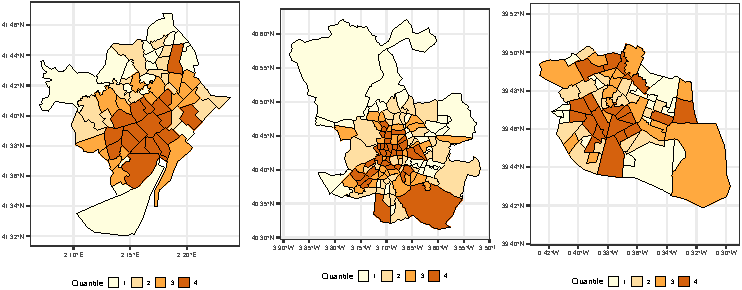
\includegraphics{EPB_files/figure-latex/unnamed-chunk-1-1.pdf}
\caption{\label{fig:all-polygons}Quantile maps of the number of
dwellings in each neighborhood. Boundary for Madrid, Barcelona and
Valencia}
\end{figure}

There are a total of 73 neighborhoods in Barcelona, 135 in Madrid and 73
in Valencia. The sf object include an unique identifier (LOCATIONID) and
the neighborhood name (LOCATIONNAME).

\hypertarget{points-of-interest}{%
\subsection{Points of Interest}\label{points-of-interest}}

The last block of data included in the data package is a set of Point of
Interest of each city in \texttt{R} list R object. The name of the list
include the name of the city with the suffix '\_POIS'
(e.g.~Barcelona\_POIS). These lists include three elements: (i) the
coordinates of the city center, identifying the central business
district; (ii) a set of points that define the main street of each city;
and (iii) the coordinates of metro stations.

\hypertarget{anonymizing}{%
\section{Anonymizing the data set}\label{anonymizing}}

To comply with Spanish regulations, two variables are slightly modified
to preserve their anonymity. A masking process is apply to asking prices
and localization (coordinates).

Whit respect to the asking prices, the original values are obfuscated
with the addition or subtraction of a random percentage of their
original values ranging from -2.5\% to +2.5\%. Since asking prices are
usually multiples of 1,000, after the first price modification, the
prices was aligned to multiples of 1,000.

\begin{algorithm}[!ht]
 \KwData{all idealista listings}
 \KwResult{all idealista listings with masked coordinates}
 initialization\;
 \For{each listing L}{
  take geographical location of L as $(X,Y)$
  \Repeat{this stop condition}{
    take a random angle $\alpha$ from 0 to 360 degrees
    take a distance $R$ as a random value from 30 to 60 meters
    determine a new point $(X',Y')$ calculated as a point located $R$ with the angle $\alpha$
  }
  set $(X',Y')$ as the new location for the listing L
 }
 \caption{Coordinate displacement process for anonymisation purposes}
 \label{algo:coordinates-displacement}
\end{algorithm}

With respect to the dwelling localization, a spatial masking process was
implemented with the intention of keeping spatial properties of the
original data set. The coordinates of each listing were displaced using
a stochastic procedure. Effectively, the listings were recorded using
coordinates contained in a maximum and minimum displacement circles, as
shown in Figure \ref{fig:Anonymizing} (left). To preserve membership in
a neighborhood, the spatial masking procedure was constrained to ensure
that the masked coordinates are in the original neighborhood of the
listing.

The Algorithm \ref{algo:coordinates-displacement} iteratively displaces
the coordinates of each listing with a minimum distance and a maximum
distance with the restriction that the new coordinates do not fall in a
different neighborhood. This ensures that neighborhood attributes are
preserved.

Figure \ref{fig:Anonymizing} (rigth) shows the histogram of
displacements in meters for all listings in the city of Valencia; the
average distance between the original and masked coordinates is 45
meters.

\begin{figure}

{\centering 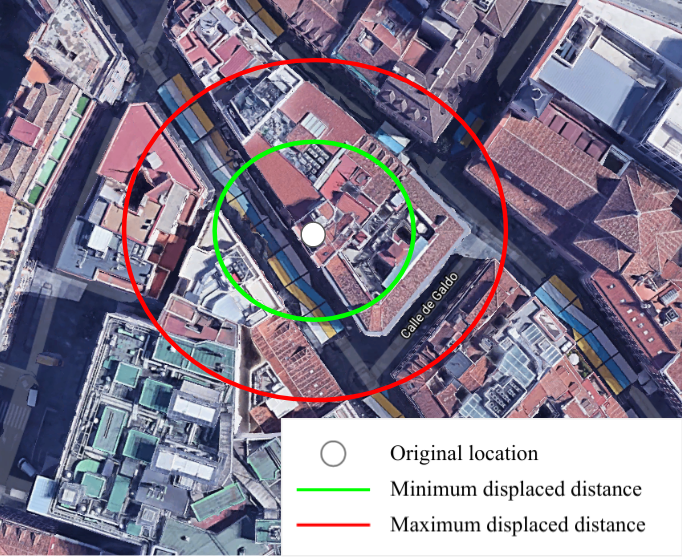
\includegraphics[width=0.29\linewidth,height=0.2\textheight]{EPB_files/points-moved-image} 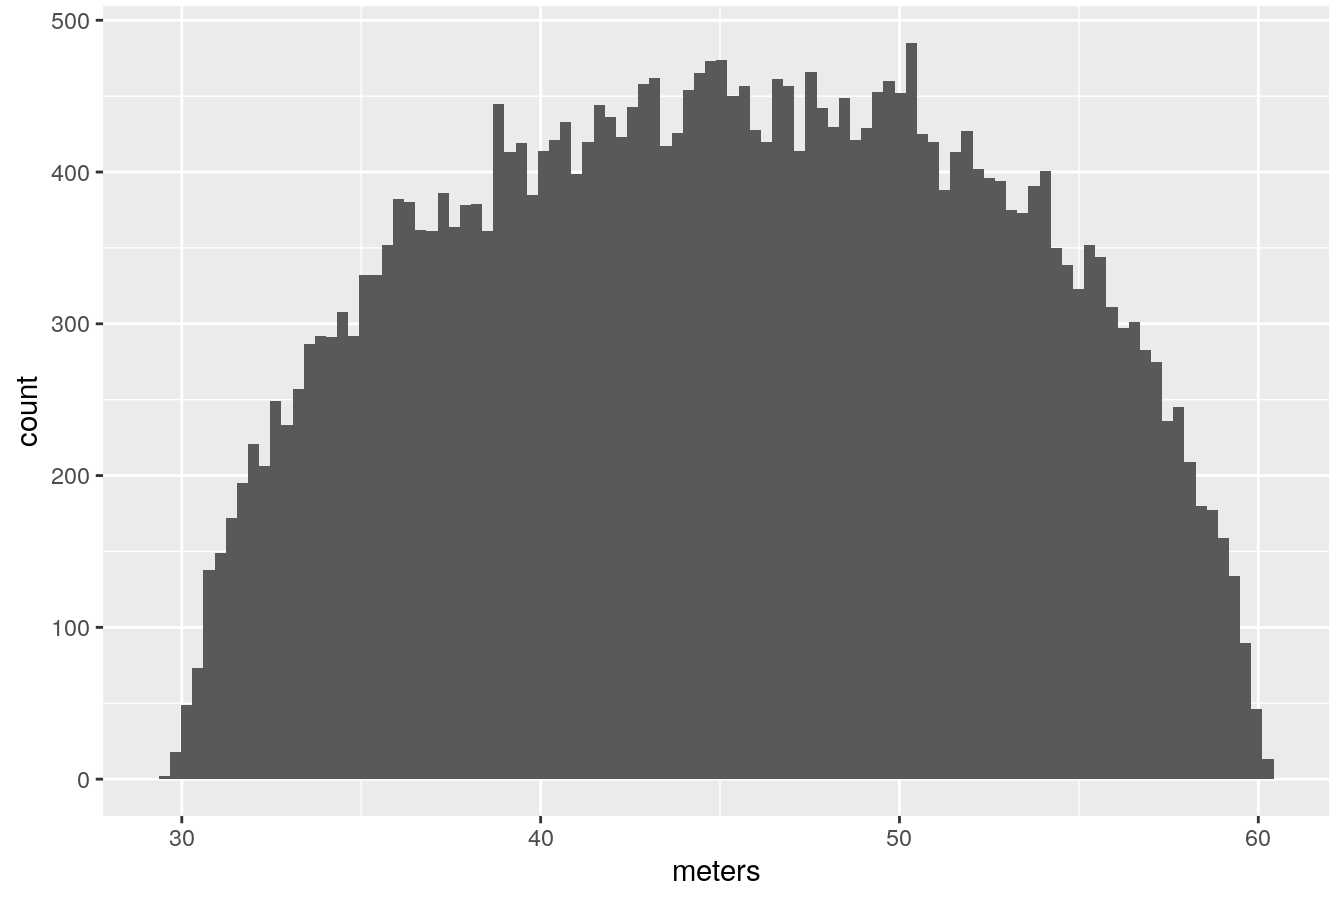
\includegraphics[width=0.37\linewidth,height=0.2\textheight]{EPB_files/coordinates-valencia} 

}

\caption{\label{fig:Anonymizing}(Left) Masking coordinates. Spatial range. (Rigth) Coordinate displacement in meters Valencia}\label{fig:unnamed-chunk-2}
\end{figure}

\hypertarget{conclusion}{%
\subsection{Conclusion}\label{conclusion}}

The data set present in this paper is excellent for applying hedonic
models with spatial effects, identifying housing submarkets, applying
machine learning techniques, etc..

\hypertarget{declaration-of-competing-interest}{%
\section{Declaration of Competing
Interest\}}\label{declaration-of-competing-interest}}

Author One and author Two are employed by idealista. They have been
granted permission to share the data presented in this article. None of
the authors have known competing financial interests or personal
relationships which have, or could be perceived to have, influenced the
work reported in this article.

\hypertarget{acknowledgments}{%
\section{Acknowledgments}\label{acknowledgments}}

The authors wish to thank Alessandro Galesi for their support in the
paper revision and Juan Ramon Selva for collecting and cleaning the
spatial data. This work has been partially funded by the Spanish
Ministry of Economy and Competitiveness Grants PID2019-107800GB- 100

\bibliographystyle{sageh}
\bibliography{bibEPB.bib}


\end{document}
